% Supplementary material — "Aligned but Inert"
% BUILD:  pdflatex supp; bibtex supp; pdflatex supp; pdflatex supp
%
% Every number here is computed by a script in the released repository from a committed
% per-case result file. Section S1 gives the file path for each table.
\documentclass[10pt,twocolumn,letterpaper]{article}

\usepackage[review,applications]{wacv}
%
% --- inline annotations
%
\newcommand{\red}[1]{{\color{red}#1}}
\newcommand{\todo}[1]{{\color{red}#1}}
\newcommand{\TODO}[1]{\textbf{\color{red}[TODO: #1]}}
% --- disable by uncommenting  
% \renewcommand{\TODO}[1]{}
% \renewcommand{\todo}[1]{#1}



%
% --- architecture figure (Fig. 1) and table rules
%
\usepackage{tikz}
\usetikzlibrary{arrows.meta,positioning,fit,backgrounds,calc}
\usepackage{booktabs}
\usepackage{amsmath,amssymb}


\definecolor{wacvblue}{rgb}{0.21,0.49,0.74}
\usepackage[pagebackref,breaklinks,colorlinks,allcolors=wacvblue]{hyperref}

\def\wacvPaperID{2592}
\def\confName{WACV}
\def\confYear{2027}

\newcommand{\casfg}{\mathrm{CAS}_{\mathrm{fg}}}
\DeclareMathOperator*{\argmax}{arg\,max}

% Supplementary numbering: S1, S2, ... and Table S1, Figure S1.
\renewcommand{\thesection}{S\arabic{section}}
\renewcommand{\thetable}{S\arabic{table}}
\renewcommand{\thefigure}{S\arabic{figure}}

\title{Aligned but Inert: Concept Bottlenecks in Dense Prediction,\\
       and How to Make Them Causal\\[4pt]
       \large Supplementary Material}

\author{Anonymous WACV submission\\
Paper ID \wacvPaperID\\
}

\begin{document}
\maketitle

\noindent
This supplement gives the implementation detail needed to reproduce the paper, the full
version of every table the paper summarizes, and the results the paper mentions but had no
room to tabulate---including the two where our own method loses. Section references of the
form ``Sec.~4'' point into the main paper; ``Sec.~S1'' points here.

\section{Implementation and reproducibility}
\label{sec:impl}

\paragraph{Data.}
BraTS 2024 adult glioma. Four co-registered modalities (T1n, T1c, T2w, T2f), skull-stripped
and interpolated to $1\,\mathrm{mm}^3$ by the challenge organizers. Native labels
$\{0,2,4\}$ are remapped to $\{$0:Background, 1:NCR, 2:Edema, 3:ET$\}$. Each modality is
$z$-scored over its non-zero voxels, then a $128^3$ patch is taken. The split is
patient-wise $75/12.5/12.5$ with seed $42$, giving $n_{\mathrm{test}}{=}168$. It is our own
split, so absolute Dice is not comparable to BraTS leaderboard results; every comparison in
the paper is within-split.

\paragraph{Backbones.}
Two, both from MONAI. \emph{SegResNet} is the headline backbone and carries every
configuration comparison. \emph{Swin}~+~UNETR decoder is the backbone on which the failure
was first diagnosed; its encoder is initialized from MONAI's self-supervised
\texttt{model\_swinvit.pt}, which requires three key remappings (strip the \texttt{module.}
prefix from DataParallel, rename \texttt{mlp.fc1/fc2} to \texttt{linear1/linear2} for
MONAI~1.5, and inflate \texttt{patch\_embed.proj.weight} from 1 to 4 input channels). All
126 encoder keys load.

\paragraph{Module.}
$K{=}4$ concepts, bottleneck $192\times16^3$ ($4096$ tokens of width $192$). The router is
linear plus $K$ learnable prototypes with a learnable temperature; experts are pre-norm
residual MLPs. Training uses soft dispatch, inference hard dispatch.

\paragraph{Optimization.}
AdamW, learning rate $10^{-4}$ with cosine decay, weight decay $10^{-5}$, gradient clip
$1.0$, mixed precision, $80$ epochs. Batch size $1$ with $4$ gradient-accumulation steps
(effective batch $4$); gradient checkpointing is on, which is what makes the model fit in
$16$\,GB. Runs were performed on a single T4 and a single L4.

\paragraph{Curriculum and loss weights.}
$\mathcal{L}=\mathcal{L}_{\text{seg}}+\lambda_1\mathcal{L}_{\text{align}}
+\lambda_2\mathcal{L}_{\text{div}}+\lambda_3\mathcal{L}_{\text{ent}}
+\lambda_4\mathcal{L}_{\text{bnd}}$, with $(\lambda_1,\lambda_2,\lambda_3,\lambda_4)$ set by
phase (Table~\ref{tab:curriculum}). $\mathcal{L}_{\text{align}}$ is a foreground-only focal
BCE with $\gamma{=}1.0$ and per-concept weights $[1,3,1,1]$, which up-weights NCR because it
is by far the scarcest concept at $16^3$; an additional contrastive term of weight $0.3$
separates NCR from ET, the pair the router confuses most. $\lambda_3$ is capped at $0.01$:
larger values push routing toward uniform and destroy $\casfg$.

\begin{table}[t]\centering\footnotesize
\setlength{\tabcolsep}{4pt}
\caption{Three-phase curriculum. $\lambda_1$ is zero during warm-up, which is the default we
inherited; ablation A4 (Sec.~\ref{sec:ablations}) shows it is not actually required.}
\label{tab:curriculum}
\begin{tabular}{lcccccc}
\toprule
phase & epochs & $\lambda_1$ & $\lambda_2$ & $\lambda_3$ & $\lambda_4$ & $\tau$ \\
\midrule
warm-up     & 1--10  & $0.0$ & $0.5$ & $0.00$ & $0.0$ & $2.0$ \\
alignment   & 11--60 & $1.0$ & $0.5$ & $0.01$ & $0.3$ & $1.0$ \\
refinement  & 61--80 & $1.0$ & $0.1$ & $0.01$ & $1.0$ & $0.5$ \\
\bottomrule
\end{tabular}
\end{table}

\paragraph{The three configurations.}
All three share backbone, losses, curriculum, optimizer, split and seed, and differ only in
the switches below, so every comparison isolates the architectural change.

\begin{table}[t]\centering\footnotesize
\setlength{\tabcolsep}{3pt}
\caption{What separates the configurations. Nothing else differs.}
\label{tab:configs}
\begin{tabular}{lccc}
\toprule
& expert & skip gate $\alpha$ & additive \\
\midrule
NATURAL & $h+c_k(h)$ & $1.0$ & no \\
GATED   & $c_k(h)$   & $0.5$ & no \\
\textbf{DIRECT} & $h+c_k(h)$ & $1.0$ & \textbf{yes}, $\lambda{=}1$ \\
\bottomrule
\end{tabular}
\end{table}

\paragraph{Where each number comes from.}
Scripts are \texttt{pipeline/routing\_intervention.py} (Test~1),
\texttt{pipeline/expert\_diagnostics.py} (Test~2 and expert statistics),
\texttt{pipeline/linear\_probe.py} (Test~3), \texttt{pipeline/evaluate.py} (Dice,
$\casfg$, AUROC, ECE) and \texttt{pipeline/error\_detection.py} (Sec.~\ref{sec:uncertainty}).
Each writes a per-case CSV and a summary JSON under \texttt{evals/}; the tables here are
rendered from those files, so the paper's figures and tables cannot drift apart.

\section{The intervention, in full}
\label{sec:intervention}

The paper reports the mean off-diagonal label-flip. Table~\ref{tab:fullmatrix} gives every
cell, for both configurations and both scopes. Two things are visible here that a single
mean hides.

First, the diagonal is \emph{exactly} zero in all four matrices. This is the identity
control: forcing the tokens already assigned to $a$ through $a$'s own expert is a bit-exact
no-op, so every off-diagonal entry is attributable to re-routing rather than to the
instrumentation. Achieving this required hardening the router's logits to a one-hot for
\emph{every} token rather than only the intervened ones (Sec.~3.4); without that, an
identity intervention moves the prediction by $14.3$ logits and the control is worthless.

Second, the asymmetry the paper discusses is a property of rows, not cells. NCR is a weak
source ($0.28$--$0.31$) and a decent target ($0.51$--$0.66$) under DIRECT, and the effect
size tracks how confidently the model held the original concept.

\begin{table}[t]\centering\footnotesize
\setlength{\tabcolsep}{4pt}
\caption{Complete label-flip matrices ($n{=}168$). Rows are the source concept, columns the
target; each entry is the fraction of re-routed voxels whose predicted label became the
target. Diagonals are the identity control. The paper quotes the mean of the six
off-diagonal cells under the tumor-restricted scope.}
\label{tab:fullmatrix}
\begin{tabular}{llccc}
\toprule
& from $\backslash$ to & NCR & Edema & ET \\
\midrule
\multicolumn{5}{l}{\emph{GATED, tumor-restricted} --- mean $0.011$}\\
& NCR   & $0.000$ & $0.028$ & $0.055$ \\
& Edema & $0.007$ & $0.000$ & $0.004$ \\
& ET    & $0.013$ & $0.009$ & $0.000$ \\
\midrule
\multicolumn{5}{l}{\textbf{DIRECT, tumor-restricted} --- mean $\mathbf{0.636}$}\\
& NCR   & $0.000$ & $0.312$ & $0.280$ \\
& Edema & $0.661$ & $0.000$ & $0.772$ \\
& ET    & $0.515$ & $0.738$ & $0.000$ \\
\midrule
\multicolumn{5}{l}{\emph{DIRECT, all tokens} --- mean $0.816$}\\
\multicolumn{5}{l}{\footnotesize reported for completeness; see the scope discussion, Sec.~5.4}\\
\bottomrule
\end{tabular}
\end{table}

\paragraph{Why we quote the smaller number.}
A router sends most of the volume to background, and roughly a quarter of all tokens to the
edema expert---most of them normal tissue. Re-routing every token of a concept therefore
repaints the whole brain and reports $0.816$. That figure is real but close to tautological
under additive routing: it shows the output follows the routing everywhere. The
tumor-restricted scope measures concept control where it is clinically meaningful, and it is
also \emph{cleaner} on both controls, not merely smaller (Table~\ref{tab:scope}).

\begin{table}[t]\centering\footnotesize
\setlength{\tabcolsep}{4pt}
\caption{Restricting the scope lowers the headline and improves both controls (DIRECT,
$n{=}168$, mean over off-diagonal pairs).}
\label{tab:scope}
\begin{tabular}{lcc}
\toprule
& tumor-restricted & all tokens \\
\midrule
target class $\uparrow$    & $\mathbf{0.540}$ & $0.798$ \\
source class $\downarrow$  & $-0.544$ & $-0.514$ \\
off-target $\to 0$         & $\mathbf{0.079}$ & $0.151$ \\
outside region $\to 0$     & $\mathbf{0.005}$ & $0.016$ \\
\bottomrule
\end{tabular}
\end{table}

\section{Expert diagnostics}
\label{sec:experts}

The paper rules out expert degeneracy as the explanation for inertness.
Table~\ref{tab:experts} gives the underlying numbers for all three configurations, and they
carry a result that is easy to miss: the subtractive repair did not merely fail, it made the
experts \emph{interchangeable}. Removing the residual so that $E_k(h)=c_k(h)$ drops mean
pairwise divergence from $0.93$ to $0.16$. With a residual, each expert supplies only a
concept-specific correction and is free to differ; without one, every expert must
independently reconstruct whatever the decoder needs, so they converge on nearly the same
map. This is the clearest single piece of evidence for the paper's claim that subtractive
repairs backfire.

\begin{table}[t]\centering\footnotesize
\setlength{\tabcolsep}{4pt}
\caption{Expert statistics ($n{=}40$). Residual scale is
$\lVert E_k(h)-h\rVert/\lVert h\rVert$; divergence is
$\lVert E_a(h)-E_b(h)\rVert/\lVert h\rVert$ averaged over pairs. NATURAL is measured on Swin
($\dagger$), the backbone on which the design was first diagnosed.}
\label{tab:experts}
\begin{tabular}{lcc}
\toprule
& residual scale & pairwise divergence \\
\midrule
NATURAL$^\dagger$ & $0.59$--$0.74$ & $0.93$ \\
GATED             & ${\approx}1.01$ & $0.16$ \\
\textbf{DIRECT}   & $0.21$--$0.47$ & $0.42$ \\
\bottomrule
\end{tabular}
\end{table}

\paragraph{Ablating a two-path module.}
Under additive routing the module reaches the output twice, and each path must be ablated
separately. Table~\ref{tab:necessityfull} gives all four conditions. \emph{bypass} replaces
the module output with raw encoder features; \emph{zero\_expert} zeros the features the
decoder consumes; \emph{zero\_routing} zeros the additive term; \emph{zero} removes both.
Patching only the decoder's bottleneck input---the obvious thing to do---leaves the additive
term intact and measures a $0.09$ logit change where the true effect is $7.0$. A study using
that measurement would conclude the bottleneck is unnecessary and reject a working design.

\begin{table}[t]\centering\footnotesize
\setlength{\tabcolsep}{4pt}
\caption{Bottleneck necessity for DIRECT (per-class Dice, $n{=}40$). Removing the routing
term alone destroys the prediction; this is the same model whose inert predecessor lost at
most $3.1$ Dice to having its entire bottleneck zeroed.}
\label{tab:necessityfull}
\begin{tabular}{lcccc}
\toprule
& base & bypass & zero\_expert & \textbf{zero\_routing} \\
\midrule
NCR   & $0.483$ & $0.484$ & $0.053$ & $\mathbf{0.006}$ \\
Edema & $0.898$ & $0.477$ & $0.333$ & $\mathbf{0.418}$ \\
ET    & $0.852$ & $0.597$ & $0.428$ & $\mathbf{0.172}$ \\
\bottomrule
\end{tabular}
\end{table}

\paragraph{An interaction we cannot explain.}
Zeroing \emph{both} paths is less damaging than zeroing the routing term alone (edema
$0.801$ vs.\ $0.418$). Our best guess is that the decoder, trained to add to a routing base,
is left miscalibrated when the base is stripped but the expert path remains, whereas zeroing
both puts it in a cleaner regime. We report it because it is reproducible and we do not have
a confirmed account of it.

\section{Alignment emerges from the segmentation loss}
\label{sec:emergence}

A natural objection to $\casfg$ is that it only measures what $\mathcal{L}_{\text{align}}$
trains. Additive routing answers it directly. Because the routing logits are a term of the
output, $\mathcal{L}_{\text{seg}}$ alone trains them to be concept-aligned---so alignment
should appear during warm-up, when $\mathcal{L}_{\text{align}}$ is switched off entirely.
It does (Fig.~\ref{fig:emergence}). At epoch~10, with $\lambda_1$ still zero, DIRECT has
reached $\casfg$ $0.41$ on edema and $0.42$ on ET against $0.16$ and $0.15$ for NATURAL.
The alignment is a consequence of the architecture, not only of the supervision.

\begin{figure}[t]\centering
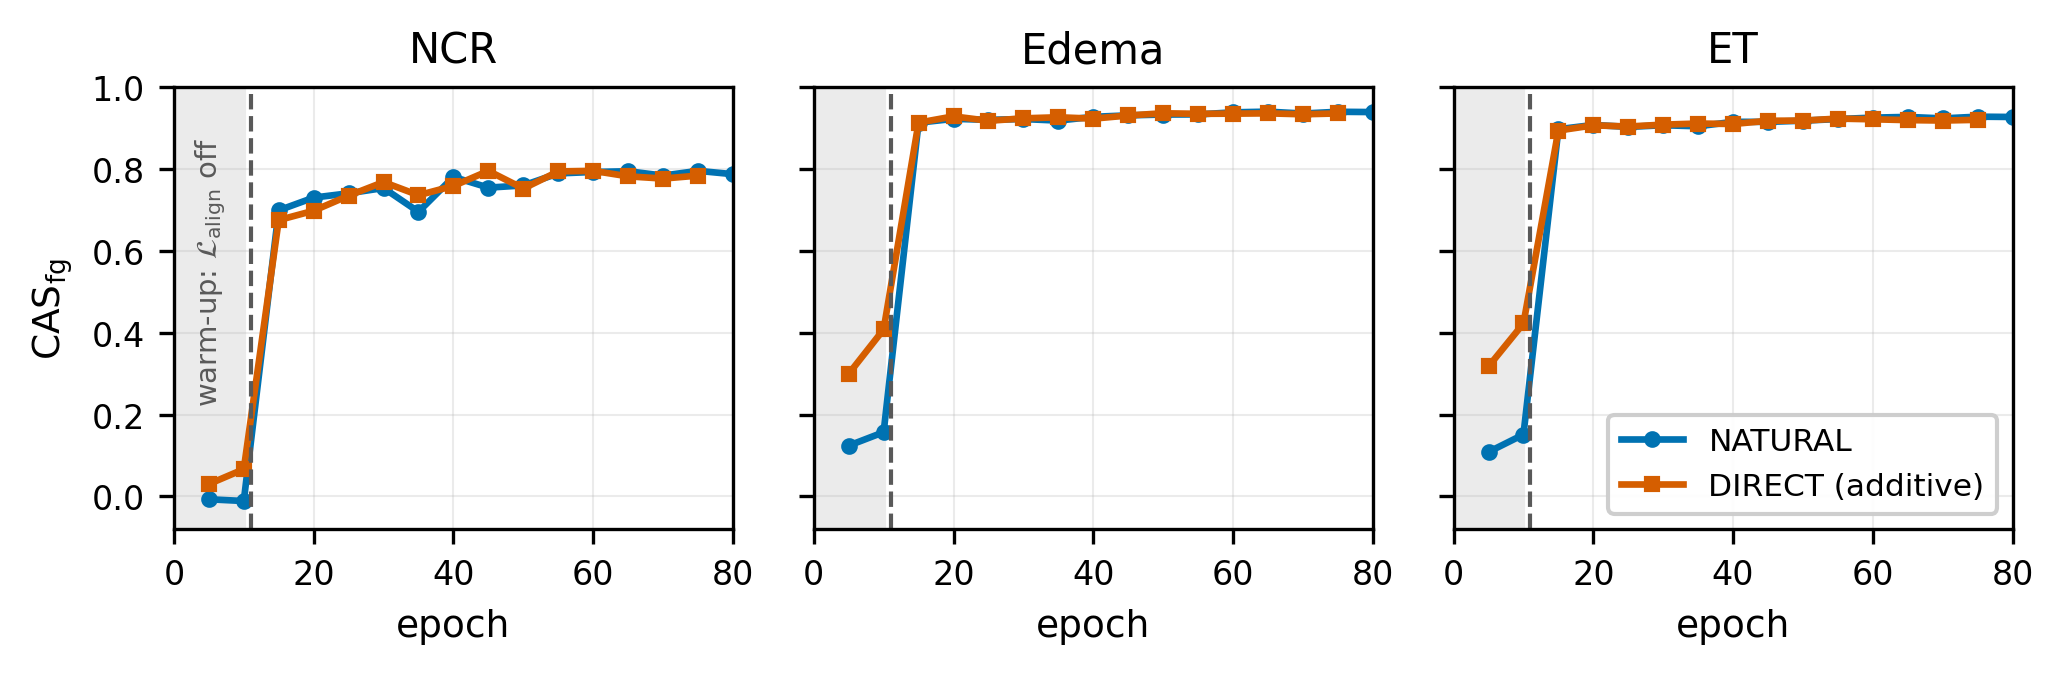
\includegraphics[width=\linewidth]{figures/fig_cas_emergence.png}
\caption{$\casfg$ during training. The shaded band is warm-up, where
$\mathcal{L}_{\text{align}}$ is off. NATURAL's routing sits near the floor until alignment
supervision switches on at epoch~11; DIRECT's climbs during warm-up, because the routing
logits are part of the output and the segmentation loss therefore trains them.}
\label{fig:emergence}
\end{figure}

\section{Post-hoc baselines: the comparison we lose}
\label{sec:baselines}

The paper concedes that post-hoc attribution wins on deletion and insertion AUC and does not
tabulate it. Table~\ref{tab:delins} gives the numbers. Integrated gradients and occlusion
reach ${\approx}0.95$ deletion, far above what routing achieves.

We read this as a statement about what the metric measures rather than a defeat. Deletion
and insertion score \emph{input sensitivity}: how fast the prediction degrades as
highly-ranked voxels are removed. A method that is optimized to find sensitive inputs will
win, and integrated gradients is exactly that. It is not a measure of whether the model's
own concept assignment is load-bearing, which is the question this paper asks and which no
saliency map can be asked at all---there is nothing in a readout to intervene on.

\begin{table}[t]\centering\footnotesize
\setlength{\tabcolsep}{4pt}
\caption{Deletion and insertion AUC against ground-truth regions (Swin, $n{=}168$; NCR
$n{=}67$, ET $n{=}163$ where the concept is present). Higher is better for both. Post-hoc
attribution wins this comparison and we report it in full.}
\label{tab:delins}
\begin{tabular}{lcccccc}
\toprule
& \multicolumn{2}{c}{NCR} & \multicolumn{2}{c}{Edema} & \multicolumn{2}{c}{ET} \\
\cmidrule(lr){2-3}\cmidrule(lr){4-5}\cmidrule(lr){6-7}
& del & ins & del & ins & del & ins \\
\midrule
Occlusion   & $0.952$ & $0.972$ & $0.942$ & $0.897$ & $0.961$ & $0.918$ \\
Int.\ grad. & $0.962$ & $0.901$ & $0.948$ & $0.898$ & $0.946$ & $0.929$ \\
Gradient    & $0.787$ & $0.461$ & $0.674$ & $0.475$ & $0.460$ & $0.411$ \\
Grad-CAM    & $0.455$ & $0.350$ & $0.392$ & $0.369$ & $0.400$ & $0.356$ \\
\bottomrule
\end{tabular}
\end{table}

\paragraph{Concept-discriminability, per concept.}
The paper reports the mean. Per concept, and taking both sides from the same run
(Swin$^\dagger$, foreground AUROC against other tumor voxels), the routing reaches
$0.854/0.891/0.872$ on NCR/edema/ET against $0.850/0.778/0.888$ for a linear probe on the
features entering the module. The probe is competitive on NCR and marginally \emph{better} on
ET; the concept machinery earns its $+0.033$ mean advantage almost entirely on edema. For
reference, SegResNet's routing reaches $0.853/0.905/0.889$, but we do not have a matched probe
for it and so do not form that comparison.

\section{Ablations}
\label{sec:ablations}

\paragraph{A1 --- no alignment loss.}
Setting $\lambda_1{=}0$ throughout collapses $\casfg$ to $-0.011/0.322/0.094$ and
concept-discriminability to $0.294/0.843/0.274$, while Dice barely moves (WT $0.905$ vs.\
$0.927$). Alignment is therefore \emph{learned}, not incidental to competent segmentation.
The same number carries the paper's uncomfortable corollary: the segmentation does not need
the alignment.

\paragraph{A4 --- no warm-up.}
Switching $\mathcal{L}_{\text{align}}$ on from epoch~1 was expected to cause expert collapse.
It does not: $\casfg$ reaches $0.666/0.932/0.927$ against $0.688/0.935/0.930$ for the full
curriculum, and Dice WT is $0.908$. With a pretrained encoder, prototype-anchored router and
a diversity term active from the first epoch, warm-up is redundant. Its only measurable
effect is a mild improvement in utilization balance. We keep it as a safe default and report
this as a robustness result rather than a justification.

\section{Uncertainty: a negative result}
\label{sec:uncertainty}

Routing entropy is a natural per-voxel uncertainty signal and we tested whether it predicts
where the model is wrong. It does not, and plain segmentation confidence---available from the
same forward pass, with no concept machinery---beats every routing-derived signal we tried
(Table~\ref{tab:errdet}). Routing ECE is $0.65$--$0.84$ across configurations, which is
poorly calibrated in absolute terms. We therefore make no uncertainty claim anywhere in the
paper and do not position routing entropy against MC-dropout or deep ensembles.

\begin{table}[t]\centering\footnotesize
\setlength{\tabcolsep}{4pt}
\caption{Predicting voxel-level model error (AUROC, $n{=}168$, mean error rate in region
$0.171$). The best routing-derived signal is $0.097$ \emph{below} plain segmentation
confidence.}
\label{tab:errdet}
\begin{tabular}{lc}
\toprule
signal & error-detection AUROC \\
\midrule
segmentation confidence & $\mathbf{0.883}$ \\
routing/decoder disagreement (soft) & $0.786$ \\
routing/decoder disagreement (hard) & $0.726$ \\
routing entropy & $0.560$ \\
\bottomrule
\end{tabular}
\end{table}

\section{Backbone transfer}
\label{sec:backbone}

Table~\ref{tab:backbones} gives both backbones on the natural design. They differ in
pretraining, capacity and accuracy, and agree on everything that matters to the paper's
argument: both align well, and both are inert. The transformer additionally shows the
placement failure in its sharpest form---its module sits at stage~2 of~5, so the two deeper
and more semantic encoder stages bypass it entirely, which is worth stating plainly because
our own first design made exactly that error while the paper it produced said ``encoder
bottleneck''.

\begin{table}[t]\centering\footnotesize
\setlength{\tabcolsep}{4pt}
\caption{The natural design on both backbones ($n{=}168$). Dice is over nested BraTS
regions; $\casfg$ and discriminability are per concept.}
\label{tab:backbones}
\begin{tabular}{lcc}
\toprule
& Swin + UNETR & SegResNet \\
\midrule
Dice WT/TC/ET       & $0.915/0.845/0.837$ & $0.927/0.883/0.869$ \\
$\casfg$ N/E/T      & $0.69/0.94/0.93$    & $0.80/0.96/0.95$ \\
concept-discrim.    & $0.872$             & $0.883$ \\
causally inert      & yes                 & yes \\
\bottomrule
\end{tabular}
\end{table}

\section{Limitations restated}
\label{sec:limits}

For convenience, the limitations declared across the main paper, collected. One dataset and
one anatomy. No reader study, so no claim that clinicians want concept-level explanations.
No plain-backbone accuracy control, so the ${\approx}1$ Dice cost is a relative figure
against the same architecture with an inert bottleneck, not the cost of adding the module to
a plain network. The NATURAL causal numbers are a $5$-case pilot on the Swin backbone; GATED
carries $n{=}168$ on SegResNet and is equally inert. A $16^3$ bottleneck makes the
explanation coarse, and NCR---tens of tokens per case---is the consistent weak spot across
every metric we report. $K{=}4$ follows the BraTS protocol and forces transition-zone tokens
into a single concept. Finally, the two leaks are properties of an architecture family
rather than of this dataset, but that expectation is untested outside the two backbones here.

\end{document}
